\section{Task 1 - Illustration of inequalities}

\newcommand{\vxbar}{\frac{1}{20}\sum_{i = 1}^{20} X_i}
\newcommand{\xbar}{\bbar{X}_{20}}

\subsection{Deriving the bounds}

Before diving into the code, I need to derive the three bounds. To skip the
math, go to \cref{sec:task_1} on page \pageref{sec:task_1}.

\subsubsection{Markov's bound}


Let $\xbar$ denote the sample mean s.t. $\xbar = \tfrac{1}{20}\textstyle
\sum_{i = 1}^{20}X_i$.

The expression I want to bound is then:
\begin{align}
  \PP{\xbar \geq \alpha}\label{eq:bound_start}
\end{align}

Since $\xbar$ is in itself a random variable, I can plug it and $\alpha$
straight into the formula for Markov's inequality to find the bound:

\begin{align*}
  % \PP{\xbar \geq \alpha} \ &\leq\ \frac{\E\left[\,\xbar\right]}{\alpha}
  \PP{\xbar \geq \alpha} \ &\leq\ \frac{\EE{\xbar}}{\alpha}
                           % &\leq\ \frac{\E\left[\,\vxbar\right]}{\alpha}\\
\end{align*}

Using linearity of the expected value and the fact that $\E\left[X\right] = p$
when $X$ is Bernoulli distributed with bias $p$:

\begin{align*}
  \PP{\xbar \geq \alpha} \ &\leq\ \frac{\tfrac{1}{20}\sum\limits_{i =
  1}^{20}\E\left[X_i\right]}{\alpha}\\
                            &=\ \frac{\tfrac{1}{20}20p}{\alpha}\\
                            &=\ \frac{p}{\alpha}.
\end{align*}

Thus Markov's bound is simply $\frac{p}{\alpha}$.

\subsubsection{Deriving Chebyshev's bound}

Let again $\xbar$ denote the sample mean. Then, start by subtracting the
expected value of $\xbar$ from either side of the inequality:

\begin{align*}
  \PP{\xbar \geq \alpha} &= \PP{\xbar - \EE{\xbar} \geq \alpha - \EE{\xbar}}\\
\end{align*}

In order to morph the expression into something that fits the form of the LHS of Chebyshev's
inequality, I need to take the absolute value of $\xbar - \EE{\xbar}$. However,
this is okay, since the resulting bound will still be a bound for the original
expression, by transitivity of the inequality operator. Thus:
\begin{align*}
  \PP{\xbar - \EE{\xbar} \geq \alpha - \EE{\xbar}}\ &\leq\ \PP{\left|\xbar -
  \EE{\xbar}\right| \geq \alpha - \EE{\xbar}}
\end{align*}
Using Chebyshev's inequality:
\begin{align*}
  &\leq\  \frac{\var{\xbar}}{\alpha - \EE{\xbar}}\\
  &= \frac{\var{\vxbar}}{\alpha - \EE{\xbar}}\\[4pt]
  &= \frac{\tfrac{1}{400}\var{\sum_{i = 1}^{20}X_i}}{(\alpha - \EE{\xbar})^2}
\end{align*}
Using independence of $X$:
\begin{alignat*}{3}
  &=\ \frac{\tfrac{1}{400}\sum_{i = 1}^{20}\var{X_i}}{(\alpha - \EE{\xbar})^2}\\
\end{alignat*}

Using $\var{X} = p(1 - p)$ when $X$ is a Bernoulli RV with bias $p$:

\begin{alignat*}{3}
  &=\ \frac{\tfrac{1}{400}\sum_{i = 1}^{20}p(1 - p)}{(\alpha -
  \EE{\xbar})^2}\\[4pt]
  &=\ \frac{\tfrac{1}{400}* 20 * p(1 - p)}{(\alpha - \EE{\xbar})^2}\\[4pt]
  &=\ \frac{p(1 - p)}{20(\alpha - \EE{\xbar})^2}
\end{alignat*}

\noindent Finally, using $\EE{\xbar} = p$, as computed earlier, I arrive at the desired
bound:
\begin{alignat*}{3}
  &=\ \frac{p(1 - p)}{20 *(\alpha - p)^2}
\end{alignat*}

\subsubsection{Deriving Hoeffding's bound}

Starting again from \cref{eq:bound_start}, subtract $\mu$ from either side of
the inequality to:

\begin{align*}
  \PP{\xbar \geq \alpha} &= \PP{\xbar -\mu \geq \alpha - \mu}
\end{align*}

Let $\eps := \alpha - \mu$. Then Hoeffding's bound is:

\begin{align*}
  \text{exp}(-2 * 20 * \eps^2) &= \text{exp}(-40 * (\alpha - \mu)^2).
\end{align*}


\subsubsection{Translating the bounds to code}

If \texttt{alphas} is a NumPy array containing alpha values and \texttt{p} is the
chosen bias, then the bounds are given in Python (using numpy vector ops) as such:

\begin{minted}{python}
markov_bounds    = p / alphas
chebyshev_bounds = (p * (1 - p) / (20 * (alphas - p)**2)).clip(0, 1)
hoeffding_bounds = np.exp(-40 * (alphas - p) ** 2)
\end{minted}

Note the use of \texttt{.clip(0, 1)} on line 2 -- this assures that none of
Chebyshev's bounds exceed 1, which for example happens for $p = 0.5$ and $\alpha
\leq 0.6$.


\subsection{Tasks 1-6 for p = 0.5}
\subsubsection{Task 1 -- Plotting empirical frequencies}
\label{sec:task_1}

I compute the empirical frequencies with:

\begin{minted}{python}
alphas    = np.arange(alpha_lo, alpha_hi + 0.05, 0.05).reshape((-1, 1))
samples   = np.random.binomial(np.ones(n * 20, dtype = int), p).reshape((-1, 20))
emp_freqs = (samples.mean(1) >= alphas).sum(1) / n
\end{minted}

\noindent And plot them in \cref{fig:task_1_a} on page \pageref{fig:task_1_a}.

\subsubsection{Task 2 - Granularity of alpha}
\label{sec:task_2}

For each $X_i$ we have $X_i \in \{0, 1\}$, meaning the possible values for
$\textstyle \sum_{i = 1}^{20} X_i$ are the numbers $\{0, 1, \dots, 20\}$, and thus
the possible values for the mean are:

$$\{\tfrac{n}{20}\ :\  n \in \{0, 1, \dots, 20\}\}\ =\ \{0, 0.1, 0.15, \dots, 1\}.$$
Hence we have:
\begin{align*}
  X_i \geq \alpha \implies X_i \geq \frac{\left\lceil20\alpha\right\rceil}{20}
\end{align*}

\noindent for all $\alpha \in [0, 1]$.

\bigskip

Additionally, we only care about $\alpha \geq 0.5$, since Chebyshev's inequality
does not hold when $\alpha < 0.5$, since here you have an epsilon that
non-positive (in fact this also happens for $\alpha = 0.5$).

\subsubsection{Tasks 3, 4, 5, 6 for p = 0.5 -- Plots and discussion}

\begin{figure}[H]
  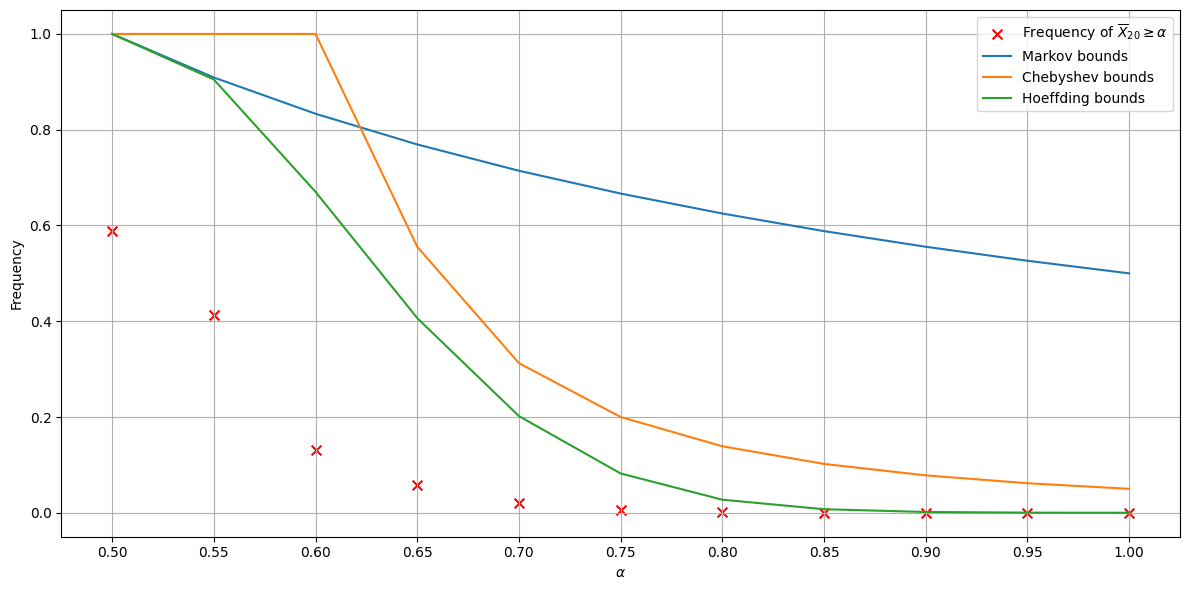
\includegraphics[width=\textwidth]{figures/task_1_a.png}
  \caption{\footnotesize Markov's, Chebyshev's, Hoeffding's bounds for $p =
  0.5$,
  $\alpha \in \{0.5, 0.55, \dots, 1\}$.}
  \label{fig:task_1_a}
\end{figure}

Interestingly, for $p = 0.5$, Chebyshev's bound is larger than Markov's for
$\alpha \leq 0.6$, but this is likely due to numerical errors since for these
alpha values the bounds exceeded 1 before truncation. Across the rest of the
plot, ie. for $\alpha > 0.6$, the bounds behave as expected, with Hoeffding's
bounds being smaller than Chebyshev's bounds, and Chebyshev's bounds being
smaller than Markov's. 

For all values of $\alpha$, the empirical frequencies are bounded from above by
all three bounds.

\subsubsection{Task 7 for p = 0.5 -- Exact probabilities}
\label{sec:exact_probs}

I want to compute the exact probability:
\begin{align*}
  \PP{\frac{1}{20} \sum_{i = 1}^{20} X_i \geq \alpha}
\end{align*}

\noindent for $\alpha = 0.95$ and $\alpha = 1$, where $X_i$ are i.i.d Bernoulli
RV's with bias $p$. In order to do so, I want to manipulate the expression such that it can be
computed using the binomial CDF.

First, scale the expression by 20:

\begin{align*}
  \PP{\frac{1}{20} \sum_{i = 1}^{20} X_i \geq \alpha} = \PP{\sum_{i = 1}^{20}
  X_i \geq 20 \alpha}
\end{align*}

Let $S_{20} = \textstyle \sum_{i = 1}^{20}X_i$. Then $S_{20}$ is a binomial
random variable from the distribution $\text{binom}(20, 0.5)$.

The CDF for the more general distribution $\text{binom(20, p)}$ is:

\begin{align*}
  \PP{S_{20} \leq k} = F_{S_{20}}(k) = \sum_{i = 0}^{k} \binom{20}{i} p^i(1 - p)^{20 - i}
\end{align*}

\noindent However, the CDF tells me the probability that $X$ is equal to or
\textit{less than} $k$. What I want to compute is:

\begin{align}
  \PP{S_{20} \geq k} &= F_{S_{20}}(20) - F_{S_{20}}(k - 1)\nonumber\\
                &= \sum_{i = 0}^{20} \binom{20}{i} p^i(1 - p)^{20 - i} - \sum_{i
                = 0}^{k - 1} \binom{20}{i} p^i(1 - p)^{20 - i}\nonumber\\
                &= \sum_{i = k}^{20} \binom{20}{i} p^i(1 - p)^{20 - i}\label{eq:binomatleastk}
\end{align}

% \begin{align}
%   \PP{S_{20} \geq k} &= 1 - \PP{S_{20} \leq k - 1}\nonumber\\
%                 &= 1 - \sum_{i = 0}^{k - 1} \binom{20}{i} p^i(1 - p)^{20 -
%                 i}\label{eq:binomatleastk}
% \end{align}

Using the above formula, I simply plug in the values $\alpha = 0.95$ and $\alpha
= 1$ for $p = 0.5$ (note that the upper bound of the sum is integral in both
cases since both $0.95 * 20$ and $1 * 20$ are integers):

\begin{align*}
  \PP{\frac{1}{20}\sum_{i = 1}^{20} X_i \geq 0.95} &= \PP{S_{20} \geq
  20 * 0.95}\\
  &= \sum_{i = 20 * 0.95}^{20} \binom{20}{i} 0.5^i * 0.5^{20 - i}\\
  &= \sum_{i = 19}^{20} \binom{20}{i} 0.5^i * 0.5^{20 - i}\\
  &= 2.00272\text{e}-5\\[12pt]
  \PP{\frac{1}{20}\sum_{i = 1}^{20} X_i \geq 1} &= \PP{S_{20} \geq
  20 * 1}\\
  &= \sum_{i = 20}^{20} \binom{20}{i} 0.5^i * 0.5^{20 - i}\\
  &= \binom{20}{i} 0.5^i * 0.5^{20 - i}\\
  &= 9.53674\text{e}-7
\end{align*}

\subsection{Tasks 1-6 for p = 0.1}

I re-do tasks 1-6 for $p = 0.1$ and $\alpha \in \{0.1, 0.15, \dots, 1\}$.

\subsubsection{Task 1 -- Plotting empirical frequencies for p = 0.1}

The empirical frequencies are computed as before -- see \cref{sec:task_1}. The
frequencies are plotted in \cref{fig:task_1_b} on page \pageref{fig:task_1_b}.

\subsubsection{Task 2 -- Granularity of alpha for p = 0.1}

The argumentation here is the same as before (please see \cref{sec:task_2}),
except here we consider all $\alpha \geq 0.1$ since those are the values of
$\alpha$ for which Chebyshev's inequality holds when $p = 0.1$ (actually it
doesn't hold for $\alpha = 0.1$, so I'm not exactly sure why we include it).


\subsubsection{Tasks 3, 4, 5, 6 -- Plots and discussion for p = 0.1}

\begin{figure}[H]
  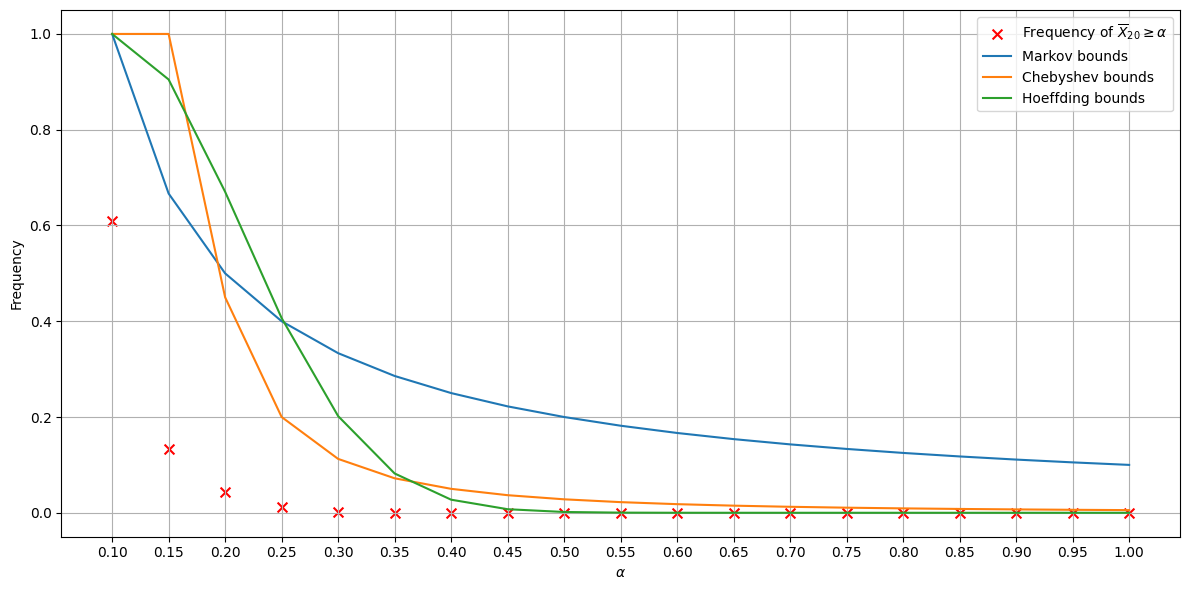
\includegraphics[width=\textwidth]{figures/task_1_b.png}
  \caption{\footnotesize Markov's, Chebyshev's, Hoeffding's bounds for $p =
  0.1$, $\alpha \in \{0.1, 0.15, \dots, 1\}$.}
  \label{fig:task_1_b}
\end{figure}

Once again we see that Chebyshev's bound exceeds 1 for $\alpha \leq 0.15$ (but
this is of course truncated to $1$ in the code). However, here it is perhaps
more interesting to note that the Markov bound binds as tight or tighter than
Hoeffding's for $\alpha \leq 0.25$, and that the Chebyshev bound binds stronger
for $\alpha \in [0.2, 0.35]$. As expected, empirical frequencies are bounded
from above by all three inequalities for all values of $\alpha$.

\subsubsection{Task 7 -- Exact probabilities for p = 0.1}

To compute the probabilities for $p = 0.1$, I will reuse
\cref{eq:binomatleastk}, ie. the formula for $\PP{S_{20} \geq k}$ that I derived
in \cref{sec:exact_probs}.

Setting $p = 0.1$, I compute the exact probabilities for $\alpha = 0.95$ and
$\alpha = 1$:

\begin{align*}
  \PP{\frac{1}{20}\sum_{i = 1}^{20} X_i \geq 0.95} &= \PP{S_{20} \geq
  20 * 0.95}\\
  &= \sum_{i = 20 * 0.95}^{20} \binom{20}{i} 0.1^i * (1 - 0.1)^{20 - i}\\
  &= \sum_{i = 19}^{20} \binom{20}{i} 0.1^i * (1 - 0.1)^{20 - i}\\
  &= 1.81e-18\\[12pt]
%
  \PP{\frac{1}{20}\sum_{i = 1}^{20} X_i \geq 1} &= \PP{S_{20} \geq
  20 * 1}\\
  &= \sum_{i = 20 * 1}^{20} \binom{20}{i} 0.1^i * 0.9^{20 - i}\\
  &= \sum_{i = 20}^{20} \binom{20}{i} 0.1^i * 0.9^{20 - i}\\
  &= \binom{20}{i} 0.1^i * 0.9^{20 - i}\\
  &= 1e-20
\end{align*}



\sectend
